\chapter{Stand der Forschung und Technik}
\label{cha:psoDomes}
	
\dictum[deutsches Sprichwort]{Ein Bild sagt mehr als 1000 Worte.}		
% -------------------------------------------------------------------------------------------------
% -------------------------------------------------------------------------------------------------
% -------------------------------------------------------------------------------------------------

\section{Grundlagen der verwendeten computergrafischen Techniken}

Dreidimensionale Objekte k\"onnen in einem Rechner nur visualisiert und verarbeitet werden, wenn ihre Struktur durch ein geeignetes Modell beschrieben wird. Ein einfaches solches Modell, auf denen die im GoCart-Projekt verarbeiteten Daten basieren, sind trinagulierte Geometrien. Sie werden im folgenden Abschnitt \ref{triGeo} n\"aher beschrieben.

In computergrafischen Systemen ist es oft erforderlich, den minimalen Abstand zwischen zwei geometrischen Objekten zu bestimmen. Um dies zu realisieren, sind effiziente Kollisionspr\"ufungsroutinen notwendig, auf die im Abschnitt \ref{colGeo} eingegangen wird.
 
In Abschnitt \ref{picking} werden kurz dreidimensionale Auswahlverfahren beschrieben.
 
\subsection{Triangulierte Geometrien}
\label{triGeo}

Eine einfache M\"oglichkeit zur Repr\"sentation von geometrischen K\"orpern sind Dreiecksnetze, sogenannte Triangulierungen. Eine Triangulierung approximiert die Oberfl\"ache eines K\"orpers durch (sehr kleine) Dreieckefl\"achen. Ein Dreieck ist ein planares Polygon und wird durch drei sogenannte Scheitelpunkte, oder eng. Vertices, definiert. Jeder dieser Scheitelpunkte beschreibt mittels x-,y- und z-Koordinaten eine Position im dreidimensionalen Raum. Triangulierungen sind ein Spezialfall polygonaler Flächenrepräsentation geometrischer K\"orper, die Objekte mit Hilfe von planaren Vielecken (Polygone) beschreiben. Das Verfahren funktioniert exakt f\"ur ebene Strukturen, bei gekrümmten Oberfl\"achen entsteht jedoch ein sogenannter Tesslierungsfehler, der umso stärker ausf\"allt, je weniger Dreiecke für die gekr\"ummte Oberfl\"ache verwendet werden. In Abbildung \ref{triangulation} ist dieses Verhalten deutlich zu erkennen: Die Triangulierung mit der h\"oheren Dreiecksanzahl wirkt an der Silhouette wesentlich runder als die mit geringerer Anzahl. 

Eine Triangulierung speichert neben den Punktdaten noch weitere Information f\"ur jedes Dreieck, wie beispielsweise Farbwerte oder sogenannte Normalenvektoren. Das sind Vektoren, die senkrecht auf der Netzoberfläche stehen und vom K\"orper  "`weg "` zeigen. Es wird zwischen Dreiecksnormalen und Punktnormalen unterschieden: Eine Dreiecksnormale ist der Vector, der orthogonal zur Dreicksfläche nach "`aussen"` zeigt. Die Punktnormale ist die Mittelung der  Dreiecksnormalen der drei Dreiecke, die an einen Scheitelpunkt angrenzen. Normalen haben in der Computergrafik verschiedenste Verwendungen, beispielsweise sind sie für essentiell f\"ur die Simulation von Oberfl\"achen in der Bildsynthese.

\begin{figure}[H]
\centerline{
	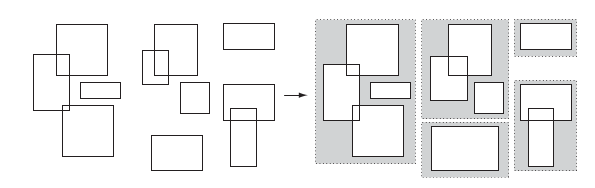
\includegraphics[width=0.7\columnwidth]{graphics/box.png}
}
\caption{Triangulierung eines Zylinders mit unterschiedlicher Dreiecksanzahl.}
\label{triangulation}
\end{figure}

Eine Triangulierung kann gespeichert und maschinell verarbeitet werden, indem f\"ur jedes Dreieck die drei Scheitelpunkte explizit gespeichert werden. Dieses Verfahren ist allerdings \"ausserst unpraktisch, da zum einen Punkte mehrfach gespeichert werden und zum anderen keine M\"oglichkeit existiert, einfach benachbarte Dreiecke zu finden. Ein besseres Verfahren sind sogenannte indizierte Polygonmengen, eng. \textit{Indexed Face Set}. Hierbei werden alle Punkte in einer Liste gehalten. Ein einzelnes Dreieck kann dann durch drei Indizes in diese Liste beschrieben werden. Auf diese Weise ist zwar keine redundante Speicherung von Punktdaten mehr n\"otig, das Problem der fehlenden Nachbarschaftsbeziehungen besteht auch bei dieser Repr\"asentation. 

Dieses Problem wird beispielsweise mit der sogenannten \textit{Winged-Edge} Datesstruktur gel\"ost, die die gesamte Topologie durch Ecken beschreibt, die Referenzen auf benachbarte Fl\"achen und Scheitelpunkte beinhaltet. 

CAD-Fahrzeugmodelle liegen liegen zunächst in triangulierter Form vor. Diese kann mit Hilfe sogenannter Triangulierungungsverfahren aus der parametrischen Repr\"asentation (z.b. Nurbs oder Bezier-Patches), mit der innerhalb von CAD-Systemen gearbeitet wird, erzeugt werden. Die Algorithmen zur Triangulierung k\"onnen unter Umst\"anden fehlerhaft triangulierte Dreiecksnetze erzeugen. Oft auftretende Probleme sind beispielsweise Selbst\"uberschneidung von Dreiecken, kleine L\"ocher, doppelte Scheitelpunkte oder sogenannte T-Scheitelpunkte. T-Scheitelpunkte sind Scheitelpunkte, die auf einer Dreieckskante liegen (siehe Abbildung \ref{tvertice}). 

\begin{figure}[H]
\centerline{
	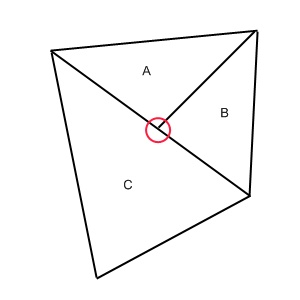
\includegraphics[width=0.4\columnwidth]{graphics/tvertices.jpg}
}
\caption{Triangulierung mit T-Scheitelpunkt.}
\label{tvertice}
\end{figure}

Einige Fehler wie doppelte Punkte oder kleine L\"ocher lassen sich durch verschiedene Bereinigungsverfahren beheben, andere, wie T-Scheitelpunkte, nicht.

\subsection{Kollisonspr\"ufung}
\label{colGeo}
 
 Unter Kollisionspr\"ufung versteht man im Allgemeinen das Erkennen von Ber\"uhrungen
oder \"Uberlappungen zweier oder mehrerer geometrischer Objekte im zwei- oder dreidimensionalen Raum.
Ein geometrisches Objekt ist hier ein K\"orper, der durch ein Polygonnetz oder
ein Freiformfl\"achenmodell beschrieben werden kann.

Es existieren eine Reihe weiterer Anwendungen, f\"ur die eine effiziente Kollisions\-pr\"ufung
unbedingt erforderlich ist:

\begin{itemize}
	\item Beim {\em Virtual Prototyping} wird die Baubarkeit der transformierten
	Einzelkomponenten des Prototyps durch Kollisionstests gew\"ahrleistet
    \cite{zachmannThesis}.
	\item In der {\em Pfad- und Bewegungsplanung} gilt es, f\"ur einen Roboter mit
	beliebigen Freiheitsgraden einen Weg von einem Start- zu einem Zielpunkt zu
	finden, ohne das dieser mit Hindernissen kollidiert \cite{lavalle}.
	\item {\em Starrk\"orper-Physiksimulationen}  f\"uhren Kollisionspr\"ufung aus,
	um in jedem Zeitschritt der Simulation zu erfassen, ob ein dynamisches Objekt mit einem
	anderen Objekt der Szene kollidiert. So k\"onnen nat\"urliche
	Verhaltensweisen starrer K\"orper, wie beispielsweise das voneinander Abprallen
	von Billardkugeln, simuliert werden.
\end{itemize}

Diese Anwendungen stellen unterschiedliche Anforderungen an ein
Kollisionspr\"ufungssystem. Zum einen m\"ussen in k\"urzerster Zeit \"Uberlappungen
zwischen dynamischen Objekten erkannt werden, zum anderen muss eine
gro"se Menge Geometrie verarbeitbar sein. Ein einfacher Ansatz, die Kollisionen
einer Szene zu finden, ist, alle Dreiecke paarweise gegeneinaner
zu testen. Dies f\"uhrt jedoch (bei  {\em n}
Szenenobjekten) zu quadratischem Aufwand:

\begin{equation}
\frac{n*(n-1)}{2} \in \mathcal O(n^2)\label{quad}
\end{equation}

So sind keine echtzeitf\"ahigen \"Uberlappungstests realisierbar! Daher muss die
Berechnungzeit mit Hilfe von Optimierungsmethoden minimiert werden. Eine Idee,
den Aufwand zu reduzieren, ist, einen Divide-and-Conquer Ansatz zu verwenden \cite{Ericson05}. 

%Sogenannte "`{\em Zwei-Phasen Algorithmen}"' wenden so einen Divide-and-Conquer Ansatz folgenderma"sen an:
%Zun\"achst wird in der "`{\em weiten Phase}"' (eng. "`{\em Broad Phase}") versucht, Paare von Objekten zu 
%finden, die miteinander kollidieren k\"onnten, weil sie r\"aumlich benachbart sind. Eine exakte  Kollisionserkennung %ist dann in der "`{\em nahen Phase}"' (eng. "`{\em Narrow Phase}") nur noch zwischen diesen Objekten erforderlich.

\begin{figure}[H]
\centerline{
	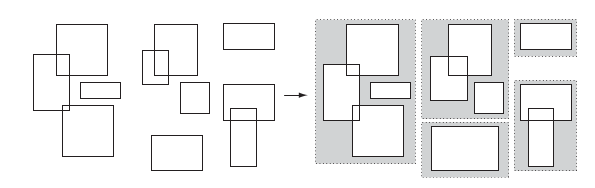
\includegraphics[width=0.7\columnwidth]{graphics/box.png}
}
\caption{Erkennung von disjunkten Objekten.}
\label{broadbox}
\end{figure}

In Abb. \ref{broadbox} sind auf der linken Seite um 11 Rechtecke auf Kollision zu pr\"ufen 55 Tests notwendig.
Nachdem in der "`weiten Phase"' 5 disjunkte Teilmengen erkannt wurden, kann die Anzahl der Tests in der "`nahen Phase"' auf 10 reduziert werden.

Ein Ansatz, die Anzahl der n\"otigen expliziten Dreiecks"-tests zu reduzieren, ist, anstelle der Dreiecke zun\"achst einen H\"ullk\"orper ({\em Bounding Volume}, kurz: {\em BV}) zu testen. Ein  H\"ullk\"orper ist ein
einfaches geometrisches Objekt wie beispielsweise ein W\"urfel oder eine Kugel, das das Objekt komplett
umh\"ullt. Die Idee ist, auszunutzen, dass die Schnitttests solcher K\"orper im Vergleich zu den eingeh\"ullten Objekten weniger aufwendig sind. So k\"onnen zun\"achst die Bounding Volumes zweier Objekte auf Kollision
getest\-et werden und nur dann, wenn dieser Schnitttest positiv verl\"auft, muss
die Dreiecksmenge der Objekte in der "`nahen Phase"' explizit gepr\"uft werden.

Die Nutzung von H\"ullk\"orpern reduziert den quadratischen Aufwand der Kollisionsp\"ufung einer Szene mit {\em n} Dreiecken soweit um einen konstanten Faktor {\em k}:
\begin{equation}
\forall k \in [0,1]:
k* \frac{n*(n-1)}{2} 
\in \mathcal O(n^2)
\end{equation}
Obwohl hierdurch der Rechenaufwand signifikant verringert werden kann, verbessert dies die Komplexit\"atsklasse des naiven Ansatzes nicht; die Anzahl der n\"otigen paarweisen Schnitttests zwischen den H\"ullen w\"achst noch immer
quadratisch bez\"uglich der Anzahl der Szenenobjekte.

Eine M\"oglichkeit, den Aufwand weiter zu reduzieren, ist die Nutzung von Hierachien aus H\"ullk\"orpern (sogenannten {\em Bounding Volume Hierachien} oder {\em BVH}). Dieser Ansatz wurde 1996 in dem Artikel "`{\em OBBTree: A Hierarchical Structure for Rapid Interference Detection}"' vorgestellt und hat seit dem die Forschung an Kollisionspr\"ufungsalgorithmen stark beeinflu"st \cite{Gottschalk}. BVH's betten die H\"ullk\"orper der Objekte rekursiv in gr\"o"sere BV's ein und ordnen diese in einer Baumstruktur an. So kann die Zeitkomplexit\"at des Algorithmus auf logarithmischen Aufwand verringert werden. Abbildung \ref{bvh} zeigt eine Hierachie weltachsenorientierter H\"ullquader, mit der f\"unf Objekte eingeh\"ullt werden.

\begin{figure}[H]
\centerline{
	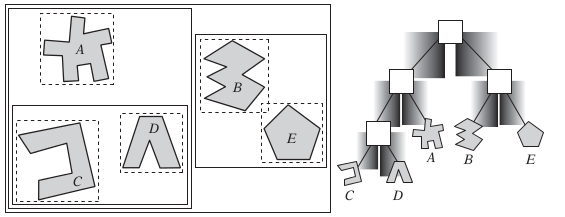
\includegraphics[scale=0.60]{graphics/bvh.png}
}
\caption{Bounding Volume Hierachie aus 5 Objekten. Auf der linken Seite wird
die Szene rekursiv umh\"ullt so dass die Baumstruktur auf der rechten Seite
daraus resultiert. }
\label{bvh}
\end{figure}

Der Ansatz rekursive H\"ullk\"orper in einer Baumstruktur anzuordnen, l\"asst
sich auch auf die Dreieckesmenge eines Objektes ausweiten. Hierbei wird die
Dreiecksmenge eines Objektes als Punktewolke interpretiert, die dann mittels
Top-Down Ans\"atzen so lange weiter unterteilt wird, bis ein Abbruchkriterium
erreicht ist. Abbildung \ref{bvho} zeigt eine solche Hierachie aus AABB's \"uber
der Dreiecksmenge eines Objektes.

\begin{figure}[H]
\centerline{
	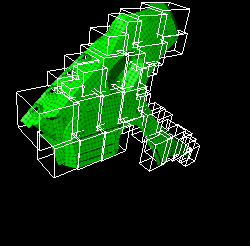
\includegraphics[scale=0.7]{graphics/BV-Hierarchie5.png}
}
\caption{Bounding Volume Hierachie \"uber den Dreiecken eines Objektes.}
\label{bvho}
\end{figure}

Um eine Szene, f\"ur die eine H\"ullk\"orperhierachie erzeugt wurde, auf Kollision zu testen, mu"s die Hierachie traversiert werden. Auf jeder Baumebene, die w\"ahrend der Traversierung besucht wird,  werden die BV's der Knoten
gegeneinander auf Kollision gepr\"uft. Wenn eine \"Uberschneidung zwischen zwei Bounding Volumes gefunden wurden, wird
die Baumsuche in diesen \"Asten fortgesetzt. Auf diese Weise wird rekursiv bis in die Blattknoten vorgegangen. Sollten die H\"ullen zweier Blattknoten \"uberlappen, kann eine Kollision zwischen den eingeh\"ullten Dreiecken bestehen, die dann in der "`Narrow Phase"' aufzul\"osen ist.

Im Rahmen dieser Arbeit wurde eine properit\"are Implementierung der frei verf\"ugbaren Bibliothek Proximity Query
Package (PQP) verwendet \cite{PQP}.

\subsection{3D-Selektion}
\label{picking}

Bei computergrafischen Anwendungen ist es oft notwendig, einen geometrischen K\"orper innerhalb einer Szene mit dem Mauszeiger zu selektieren. 

\begin{figure}[H]
\centerline{
	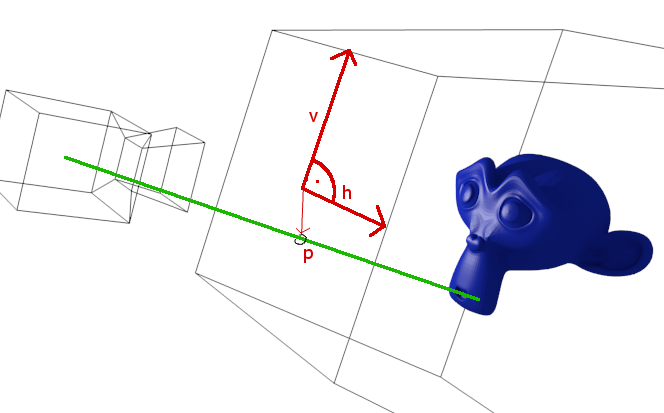
\includegraphics[scale=0.7]{graphics/raypicking.png}
}
\caption{Bounding Volume Hierachie \"uber den Dreiecken eines Objektes.}
\label{rayPicking}
\end{figure}

Eine typische Methode, dies umzusetzen, ist, einen Strahl vom Klickpunkt auf dem 3D-Ansichtsfenster der Anwendung \"uber die virtuelle Kamera in die Szene zu projizieren und zu testen,  ob der Strahl eine Geometrie schneidet (siehe Abbildung \ref{rayPicking}).
Dieses Verfahren wird als eng. \textit{Ray Casting} bezeichnet. Es hat den Vorteil, das es keine Methoden der zugrundeliegenden Grafikbibliothek benutzt und sich somit in jeder grafischen Anwendung auf die gleiche Weise verwenden l\"asst.

Um zu vermeiden, Schnittests zwischen jedem Dreieck der Szene
und dem Teststrahl durchzuführen, werden bei der Selektion mittels Ray Casting die Objektgeometrien, \"ahnlich wie bei der Kollisonspr\"ufung, durch H\"ullk\"orper ersetzt.


\section{Heuristische Optimierung}
\label{opti}

Ein Optimierungsproblem im mathematischen Sinn ist die Aufgabe, für eine Funktion eine Menge aus Eingabewerten zu finden, so das der Funktion einen minimalen (oder maximalen) Wert annimmt, wobei in der Regel eine Beschr\"ankung der Eingabewerte vorliegt. Die beste Vorgehensweise hierf\"ur h\"angt von der Art der Bewertungsfunktion ab. Ist diese beispielsweise linear, lassen sich solche Probleme mit Hilfe von Verfahren, die auf dem  sogenannten Simplex-Algorithmus basieren, effizient l\"osen.

Handelt es sich nicht um lineare Zielfunktionen, sind analytische L\"osungsverfahren meistens sehr ineffizient und das systematische Durchsuchen des L\"oesungsraums ist aufgrund der Problemgr\"o{\ss}e nicht m\"oglich. F\"ur solche Probleme werden in der Informatik oft heuristische Optimierungsverfahren eingesetzt. Diese Verfahren generieren L\"osungen anhand einer definierten Vorgehensweise und verbessern diese suzessive, bis ein Abbruchkriterium, beispielsweise die Anzahl der Iterationen, erreicht ist. 

Im Gegensatz zu analytische Verfahren beinhaltet heuristische Optimierung immer die Nutzung von Zufallswerten, beispielweise beim Simulated Annealing, das im folgenden kurz erl\"autert wird, die initialen Punkte im L\"osungsraum. Dies hat zu Folge, das heuristische Optimierungsverfahren nichtdeterministisch sind, also das bei komplexen Problemen mit mehreren lokalen Optima unterschiedliche L\"osungen gefunden werden. 

Im Folgenden werden drei heuristische Optimierungsverfahren kurz erl\"autert: \textit{Simulated Annealing}, \textit{Evolution\"are Algorithmen} und \textit{Partikelschwarmoptimierung}. 

\textbf{\textit{Simulated Annealing}} (SA, siehe \cite{Kirkpatrik}) imitiert das Abkühlverhalten von Metallen. Kühlen diese langsam ab, haben die Atome ausreichend Zeit, sich zu ordnen und eine stabile Kristallstruktur zu bilden. Der Algorithmus betrachtet einen Punkt im n-dimensionalen L\"osungsraum, der schrittweise in Richtung eines Optimums bewegt wird. Vor jeder Bewegung wird die Zielposition bewertet: Fällt die Bewertung besser aus, als die aktuelle Position, wird die Bewegung durchgeführt. Fällt sie schlechter aus, wird sie nur mit einer gewissen Wahrscheinlichkeit durchgef\"uhrt, die mit jedem Schritt sukzessive verringert wird.Diese Wahrscheinlichkeit entspricht der Temperatur des metallurgischen Abkühlungsprozesses und dient dazu, lokale Minima zu \"uberwinden.

\begin{figure}[ht]
\centering
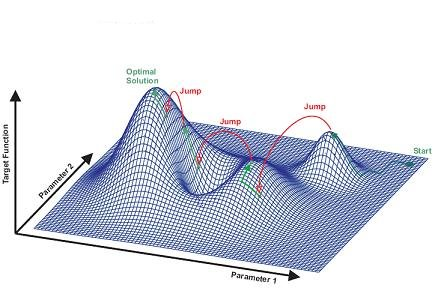
\includegraphics[width=10cm]{graphics/SimAnn.jpg}
\caption{Simulated Annealing in einem zweidimensionalen L\"osungsraum}
\label{fig6}
\end{figure}

\textbf{\textit{Evolution\"are Algorithmen} (EA)} sind eine Familie von Optimierungsverfahren, die sich das Prinzip der Selektion des Bestangepassten ("`\textit{Survival of the fittest}"') der nat\"urlichen Evolution zum Vorbild nehmen. Hierbei wird ein Punkt im L\"osungsraum als Individuum und eine Menge von Punkten als Population bezeichnet. Zu Beginn des Optimierungsverfahren wird der 
L\"osungsraum mit einer randomisierten Population "`bev\"olkert"', die zun\"achst mit einer Zielfunktion (in diesem Zusammenhang oft Fitness-Funktion) bewertet werden. Die am schlechtesten bewerteten Individuen werden verworfen, w\"arend aus den Verbliebenen die n\"achste Population durch Anwendung von sogenannten "`Evolutionären Operatoren"' erzeugt wird, beispielsweise Mutation
(leichtes Verändern eines Individuums) und Rekombination (Mischen der Gene zweier Individuen, oft auch als Crossover bezeichnet).
Dieser Zyklus aus Selektion, Crossover und Mutation wird solange wiederholt, bis ein vorgegebenes Abbruchkriterium (z. B. Anzahl der Generationen) erreicht ist.
Es werden die Hauptforschungsrichtungen Evolution\"are Programmierung (\cite{FogelAIsimEvo}), Genetische Algorithmen (\cite{GoldbergAISimEvo}) und Genetische Programmierung (\cite{KozaAIsimEvo}) unterschieden, die sich bez\"uglich der Datenstrukturen, Selektionsmethoden und der Operatoren unterscheiden.

Als \textbf{\textit{Partikelschwarmoptimierung} (PSO)} wird ein Optimierungsverfahren bezeichnet, das nach dem Vorbild nat\"urlichen Schwarmverhaltens von beispielsweise Fischen oder V\"ogeln eine L\"osung f\"ur das Optimierungsproblem sucht. Die hier beschriebene Version der PSO wurde zuerst 1995 in einer Forschungsarbeit von J. Kennedy and R. Eberhart präsentiert \cite{kennedyPSOConfPaper}. \"Ahnlich den evolution\"aren Algorithmen wird bei der Partikelschwarmoptimierung initial eine zuf\"allige  Menge vom Punkten im L\"osungsraum, die hier als Partikel bezeichnet werden, erzeugt. Der Partikelschwarm wird nun schrittweise durch den L\"osungsraum bewegt, wobei benachbarte Partikel vor jedem Schritt die beste Position, die ein Partikel bisher gefunden hat, austauschen k\"onnen. Welche Partikel miteinander kommunizieren k\"onnen wird durch die sogenannte Nachbarschaftstopologie bestimmt. 
Ein Partikel h\"alt somit zus\"atzlich zur Position $\vv{x}$ noch eine Bewegungsrichtung $\vv{v}$, die bisher beste gefundene Position als $\vv{p}_{best}$ und die beste Position seiner Umgebung als $\vv{n}_{best}$. Nach jedem Zeitschritt wird die Position und die Bewegungsrichtung (der Vektor $\vv{v}$ ist nicht normalisiert, er beinhaltet die Geschwindigkeit und Richtung) eines Partikels anhand folgender Formeln angepasst:

\begin{equation}
\vv{v}_{i,t+1} = \omega\cdot\vv{v}_{i,t}+c_{1}\cdot\vv{U}_{1}[0,1]\bigotimes(\vv{p}_{best,i,t})-\vv{x}_{i,t})
+c_{2}\cdot\vv{U}_{2}[0,1]\bigotimes(\vv{g}_{best,i,t})-\vv{x}_{i,t})
\end{equation}

\begin{equation}
\vv{x}_{i,t+1} = \vv{x}_{i,t} + \vv{v}_{i,t+1}
\end{equation}

Hierbei ist $t$ der Interationsz\"ahler, $\vv{U}_{k}[0,1]$ Zufallsvektoren und die Parameter $\omega$, $c_{1}$, $c_{1}$ bestimmen den Einflu{\ss}  der Position des vorigen Zeitschritts und der kognitiven und sozialen Komponenten.

Im Rahmen dieser Arbeit wird heuristische Optimierung benutzt, um f\"ur einen bereits ausgerichteten Zylinder H\"ohe, Radius und Rotation zu ermitteln. Dieses Problem ist nicht seperabel, d.h. einzelne Dimensionen des L\"osungsraums k\"onnen nicht oder nur begrenzt unabh\"angig voneinander untersucht werden. Dar\"uber hinaus gibt es im L\"osungsraum des Problems mehrere lokale Optima; es ist multimodal.

F\"ur die Implementierung des Optimierungsproblems wird Partikelschwarmoptimierung eingesetzt. Hierf\"ur wird ein Framework der Firma Teraport benutzt, das es erm\"oglicht, verschieden Optimierungsverfahren zu nutzen und Zielfunktionen zu implementieren.

\section{Segmentierung von triangulierten Geometrien}
\subsection{Notation und Klassifizierung von Segmentierungstechniken}
\subsection{Geometrische Eigenschaften und Unterteilungskriterien}
\subsection{Hierachisches Clustering}

\section{Automatische Featureerkennung}
\subsection{Klassifizierung von Featureerkennungstechniken}
\subsection{Subgraphisomorphismen}



